\begin{homeworkProblem}

\textbf{Markov Chain Monte Carlo for Wireless Networks.} Given a wireless network with 24 links and $0-1$ interference model, i.e., any two links are either intefere with each other or not. To describe the interference relationship between wireless links, we introduce the conflict graph model. In such model, the vertex of the conflict graph represents the wircless link. An edge between two vertioes means corresponding two links interfere with each other. The following Figure shows the corresponding conflict graph for 24-link wireless network. You are required to find the maximum independent set of the conflict graph, i.e., the largest set of wireless links that can simultancously transmit without interferences. Design the algorithm by MCMC method and evaluate your algorithm.
\begin{itemize}
\item Show your MCMC Design with a discrete Markow chain. Use both theory and simulation results to justify your algorithms.
\item Show your MCMC Design with a continnous Markov chain. Use both theory and simulation results to justify your algorithms.
\item Discuss the pros and cons for such chains.
\end{itemize}

\begin{figure}[h]
    \centering
    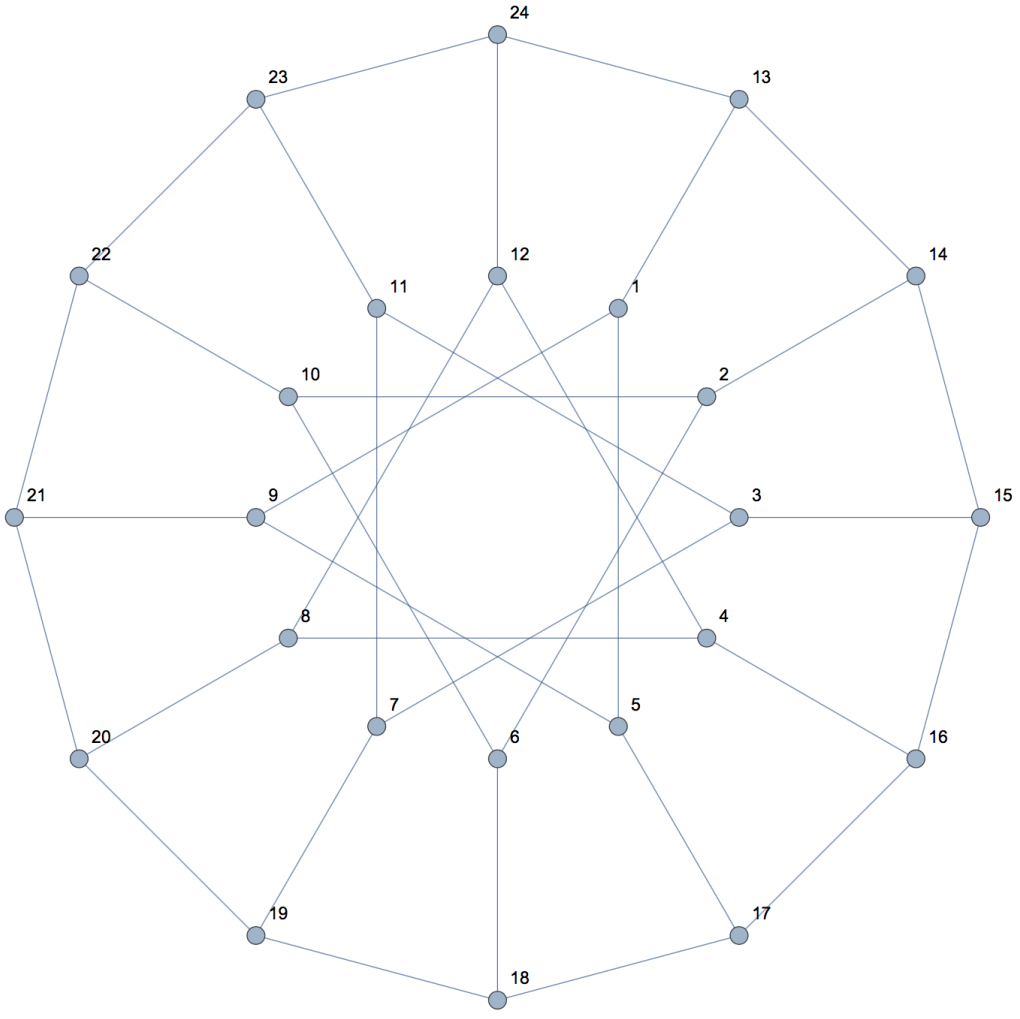
\includegraphics[width=0.5\textwidth]{./figure/p14/graph.png}
\end{figure}

\solution

(a) Discrete time Markov Chain: \\
The independent set problem is similar to the Knapsack problem: use a binary sequence to represent whether choose the link or not. And each time we randomly flip a bit in the sequence, if the new sequence does not satisfy the independent set constraint, stay at the current state, otherwise go to the new state, this is obviously a reducible Markov chain, and its stationary distribution $\pi$ is the uniform distribution.

Then, let the value function $V(x)$ be the number of selected links of the state $x$. According to the Metropolis-Hastings algorithm, the acceptance rate for the transition to $y$ is
$$a_{x,y}=e^{\beta\left(V(y)-V(x)\right)}$$
Then we just need to check the samples with largest value, i.e. the maximum indenpendent set.

The initial state is set to be an all 0 sequence, the factor is set to be
$$\beta(t)=C\cdot \log(t+1)$$
Where $C=\dfrac{1}{\log\left(\frac{T}{2}\right)}$, $T$ is the total number of steps.

After simulation $10000$ steps, the sampled maximum size of the independent set is $9$, and it sampled 65 different sequences. The first sampled sequence is: 010010100001101001010100, and it is verified to be a correct solution.

(b) Continuous time Markov Chain: \\
It is mostly same to the discrete time Markov chain, but the time is continuous, and the embedded chain has no self-transition. Thus, when considering the transition for state $x$ , we need to find out all valid transitions $y\in\N(x)$, then randomly select a transition from $\N(x)$. And there is no other difference to the discrete time Markov chain. Actually, we should set a transition rate to get the transition time intervals, but we do not need to use the time, so it is ignored.

After simulation $10000$ steps, the sampled maximum size of the independent set is $9$, and it sampled 99 different sequences. The first sampled sequence is: 110000010010001010101001, and it is verified to be a correct solution.

(c) 1. Discrete time Markov Chain: \\
Advantages: It is simple to implement, at each step, a single bit is randomly flipped. One only needs to check if the new state satisfies the independent set constraint and then directly apply the Metropolis-Hastings acceptance criterion.

Disadvantages: It may have a low acceptance rate, and stay in the origin state, the chain may explore the valid state space slowly, leading to a relatively small number of distinct sampled states. In a total of 10000 samples, only 65 different optimal states is observed.

2. Continuous time Markov Chain: \\
Advantages: The embedded chain allows transitions only to valid neighboring states chosen at random, ensuring that each transition results in a state change. In a total of 10000 samples, 99 different optimal states were observed, which is beneficial for finding the global optimum.

Disadvantages: It requires enumerating all valid neighboring states of the current state and then randomly selecting one among them, which can be slightly more complex in terms of coding and computation.

\end{homeworkProblem}

\newpage